\documentclass[../main/main.tex]{subfiles}

\begin{document}

\section{overview}

\begin{itemize}
\item limb-darkening scattering exercise we did during the course. 
— You can look into your notes from that, and I attach here also a sample program which you can use a base. 

\item After you have familiarised yourself with this, you can start to think bout how you would go about to extend this to a 3D setting (assuming isotropic scattering). 

\item (As prep for Monte-Carlo school) here is a script computing a UV resonance P-Cygni line in spherically symmetric wind with v beta-law. At top of routine, a few exercises are given, where you can modify and play around with code. Monte-Carlo program which computes a UV resonance spectral line from a fast outflowing spherically symmetric stellar wind (if you were not cc’d on that email, let me know so that I can send you the files as well). At the top of that little script, there are a few suggestions for exercises (additions) you could do to that program, in order to learn a bit more about the general workings of Monte-Carlo radiative transfer in this context.  
— So that might be a good idea for you to do as well !   (And you can also ask the others in the group for some tips etc. then.) 

\item Some background reading: 
\begin{itemize}
\item Attached mc manual by Puls. 
\item Paper by Sundqvist+ 2010 (Appendix, I think). 
\end{itemize}

\item organise meeting

\end{itemize}

\section{questions}
\begin{itemize}
\item pcyg.f90: what is the paramter $p$?
\item what is Sobo-distribution?
\item what is meant by Eddington limb-darkening?
\item Sundqvist+2009: slice: what is the geometry?
\end{itemize}

\section{Solved questions}
\begin{itemize}
\item Sundqvist + 2009: what is thermal velocity (see Wikipedia)
\item what is line force, appears in Sundqvist + 2009 (see explanation Dylan)
\item what is a flux limiter? (see course notes)
\item what is cross section of scattering (see Wikipedia)
\item Puls: p.26: how does the Milne equation appear? (see library book)
\end{itemize}

\newpage
\section{pcyg.f90}
\subsection{Overview of variables}
\begin{center}
\centering
{\tabulinesep=1.5mm
\begin{tabu}{|c|c|c|}
\hline 
name & explanation & scope \\ \hline \hline

\multicolumn{3}{|c|}{\cellcolor{orange} paramaters} \\ \hline
xk0 & \\ \hline
alpha & \\ \hline
beta & \\ \hline \hline

\multicolumn{3}{|c|}{\cellcolor{orange} start frequency of the photon} \\ \hline
xstart & start frequency & \\ \hline
vmin & & \\ \hline
vmax  & & \\ \hline

\multicolumn{3}{|c|}{\cellcolor{orange}angle of the photon} \\ \hline
xmuestart & start angle \\ \hline
xmuein & incident angle \\ \hline
xmueou & outward angle \\ \hline
\cellcolor{yellow} pstart & impact parameter \\ \hline
xnew & new photon frequency \\ \hline \hline

\multicolumn{3}{|c|}{\cellcolor{orange} optical depth} \\ \hline
tau & optical depth \\ \hline

\multicolumn{3}{|c|}{\cellcolor{orange} number of photons admin} \\ \hline
nphot & number of photons \\ \hline
nin & photons scattered back into core & \\ \hline
nout & photons escaped & \\ \hline \hline

\multicolumn{3}{|c|}{\cellcolor{orange} functions} \\ \hline
func & velocity profile \\ 
	& r & distance from center of star \\ \hline
	
xmueout & sign of outwards angle & \\ 
& xk0 & \\ 
& alpha & \\ 
& r & \\ 
& v & \\ 
& sigma & \\ \hline
\end{tabu}}
\end{center}
Finally the plot contains flux(i)-freq(i)

\newpage
\subsection{Exercises}
\subsubsection{Original code}
In original version of the code, all photons are released radially from photosphere, thus $\texttt{xmuestart} = 1$

\begin{figure}[!htp]
\centering
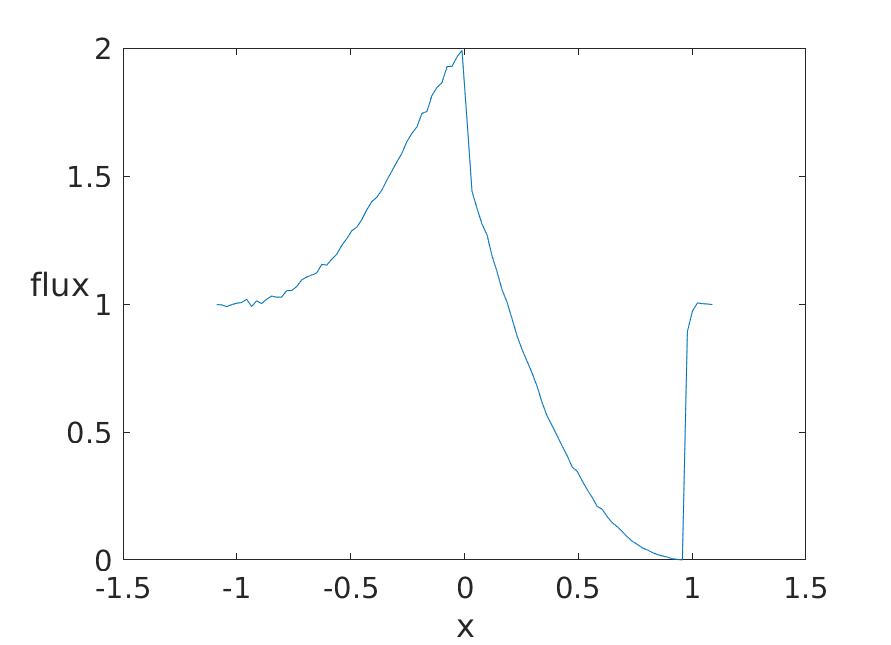
\includegraphics[width=0.5\textwidth]{../../introductory_exercises/P_Cygni_profile_UV_resonance/npot6xk0100alpha0beta1test0.png}
\caption{Original version of the code}
\end{figure}

\subsubsection{First adaption: what if all photons are released radially from photosphere?}
\begin{figure}[!htbp]
\centering
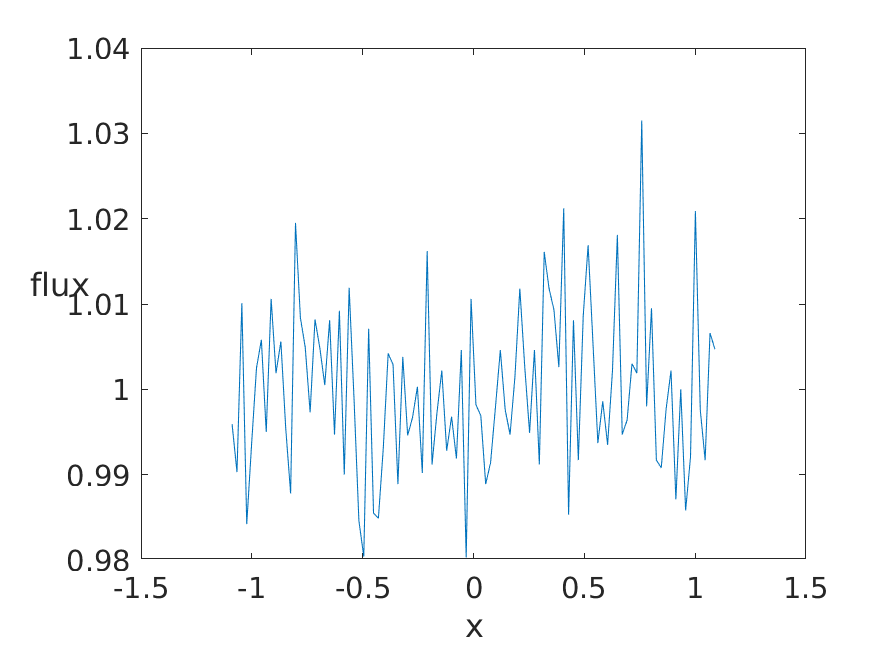
\includegraphics[width=0.5\textwidth]{../../introductory_exercises/P_Cygni_profile_UV_resonance/npot6xk0100alpha0beta1test1.png}
\caption{First adaption}
\end{figure}

\subsubsection{Second adaption: isotropic scattering}
\begin{figure}[!htp]
\centering
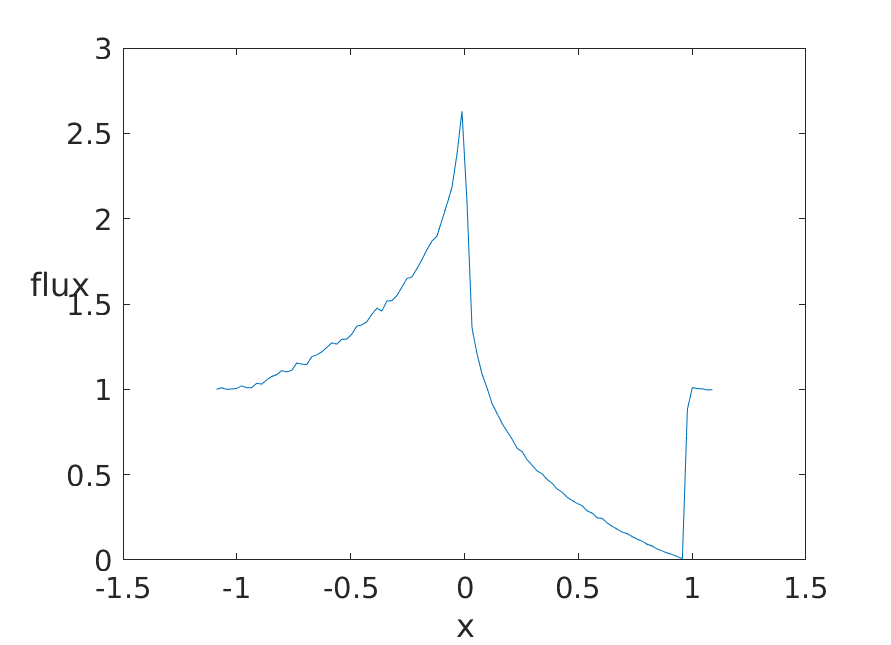
\includegraphics[width=0.5\textwidth]{../../introductory_exercises/P_Cygni_profile_UV_resonance/npot6xk0100alpha0beta1test2.png}
\caption{Second adaption}
\end{figure}

\newpage
\subsubsection{Third adaption: introduction of Eddington limb-darkening}
\paragraph{Eddington limb darkening}
\begin{itemize}
\item the source function $S= <I> = a + b\tau_{\nu}$ with $a= \frac{\sigma}{2 \pi}T_{eff}^4$ and $b = \frac{3 \sigma}{4 \pi}T_{eff}^4$
\item solve the equation
\item this yields $\frac{I(\theta)}{I(0)} = \frac{a+b\cos(\theta)}{a+b} = \frac{2}{5} + \frac{3}{5}\cos(\theta)$
\end{itemize}
\begin{figure}[!htp]
\centering
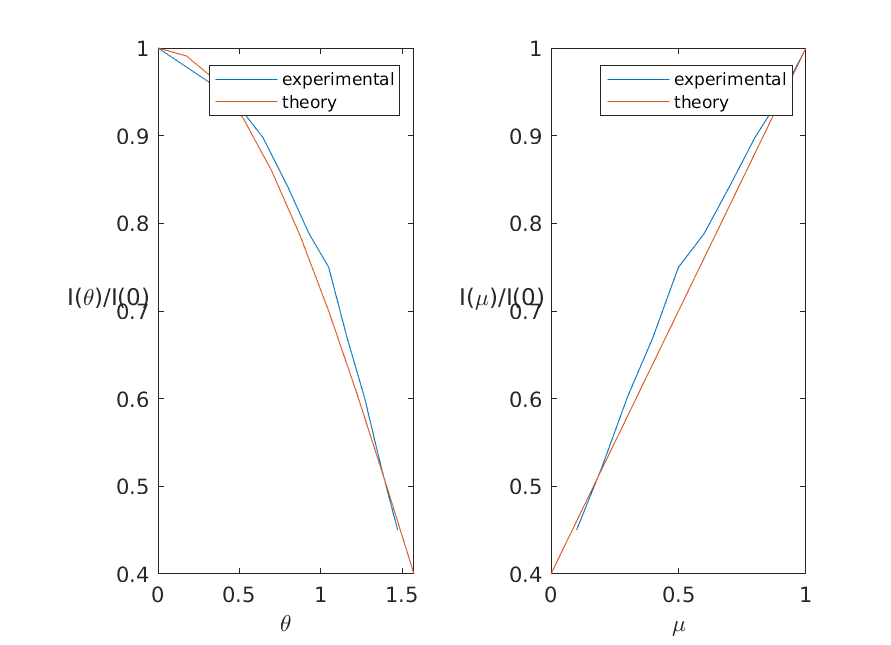
\includegraphics[width=0.7\textwidth]{../../introductory_exercises/P_Cygni_profile_UV_resonance/Eddington_limb_darkening.png}
\caption{Second adaption}
\end{figure}

\subsubsection{Fourth adaptaion: photospheric line-profile }
.

\newpage
\section{Glossary}
\begin{itemize}
\item (spectral) line-force: 

\item SED (spectral energy distribution)

\end{itemize}


\newpage
\section{Very broad introduction: Radiation Hydrodynamics}
The material here originates from the master thesis of Nicolas Moens and the course notes \textit{Introduction to numerical methods for radiation in astrophsyics} from professor Sundqvist. 

\paragraph{Heat flux}
diffusion equation $u_t = u_{xx}$. The flux  

\paragraph{Specific intensity and its angular moments}

\begin{center}
\centering
{\tabulinesep=1.5mm
\begin{tabu}{|c|c|}
\hline 
specific intensity & $\Delta \epsilon = \boxed{I_{\nu}} A_1 A_2/r^2 \Delta \nu \Delta t$ \\ \hline
energy density & $E = \frac{1}{c} \iint I_{\nu} d\nu d\Omega$ \\ \hline
flux vector & $F = \iint I_{\nu}n d\nu d\Omega$ \\ \hline
pressure tensor & $P = \iint I_{\nu} nn d\nu d\Omega$ \\ \hline
mean intensity & $J_{\nu} = \frac{c}{4 \pi} E_{\nu}$ \\ \hline
Eddington flux & $H_{\nu} = \frac{1}{4 \pi} F_{\nu}$ \\ \hline
Eddington's K & $K_{\nu} = \frac{c}{4 \pi}P_{\nu}$ \\ \hline
\end{tabu}}
\end{center}



\paragraph{RHD equations}
The full RHD equations consist of 
\begin{itemize}
\item five partial differential equations
\item one HD closure equation, e.g. (i) variable Eddington tensor method or (ii) flux limited diffusion
\end{itemize}

\paragraph{Eddington factor}
In general, the Eddington factor is a tensor, for 1D systems it is reduced to a scalar.
\begin{equation}
f_{\nu} = \frac{K_{\nu}}{J_{\nu}} = \frac{P_{\nu}}{E_{\nu}}
\end{equation}
\begin{itemize}
\item isotropic radiation field
\item radiation field stronly peaked in radial (i.e. vertical in cartesian) direction
\end{itemize}

\paragraph{Radiation transport equations, diffusion, equilibrium}
\begin{itemize}
\item black body radiation (Planck function $I_{\nu} = J_{\nu} = B_{\nu}$
\item in general, extinction(absorption,scattering) and emission
\begin{equation}
\frac{dI_{\nu}}{ds} = j_{\nu} - k_{\nu}I_{\nu}
\end{equation}
\begin{itemize}
\item Cartesian coordinates: 
\begin{equation}
\boxed{\frac{\partial I_{n,\nu}}{\partial t}\frac{1}{c} + n \nabla I_{n,\nu} = j_{\nu} - k_{n,\nu}I_{n,\nu}}
\label{radiation_transfer_equation}
\end{equation}
\item spherical coordinates 
\item 1D-problem with only variation along z-axis $\mu \frac{dI}{dz}  = j -kI$
\item spherical symmetry $\mu \frac{\partial I}{\partial r} + \frac{1-\mu^2}{r}\frac{\partial I}{\partial \mu} = j-kI$
\item plane-parallel approximation 
\begin{equation}
\boxed{\mu \frac{d I}{dr} = j - kI} 
\label{plane_parallel_radiation}
\end{equation}
The angle $\mu$ is constant throughout the computational domain.
Dividing by $k_{\nu}$, this yields 
\begin{equation}
\mu \frac{dI}{k_{\nu} dr} =  \mu \frac{dI}{k_{\nu} dz} = S-I
\end{equation}


\end{itemize}
\item Oth moment equation: integrate Equation (\ref{radiation_transfer_equation}) over $\nu$ and $\Omega$, i.e. $\int d\nu d\Omega$. Conservation of energy
\item first multiply Equation (\ref{radiation_transfer_equation}) with $\frac{n}{c}$ and then do integration
\end{itemize}

\paragraph{Radiative Diffusion Approximation}
\begin{enumerate}
\item Black-body radiation in perfect equilibrium
\item Radiative transfer equation in the \textit{near-surface} limit.
\end{enumerate}
\underline{The approximation is the following}: replace $\boxed{I = B}$ or $I_{\nu} = B_{\nu}$, once but not twice.
\begin{equation}
I_{\nu} = B_{\nu} - \mu \frac{dB_{\nu}}{k_{\nu}dz}
\end{equation}

\underline{Derive this equation as a random walk of photons!}

\subsection{Examples of radiation (diffusion equation)}
\begin{enumerate}
\item Temperature structure in a static stellar atmosphere
\item 
\end{enumerate}

\subsection{Applications and approximations for radiative forces}
\begin{itemize}
\item definition of general radiative acceleration vector $g = \frac{1}{\rho c}\int \int n k_{\nu} I_{\nu} d\Omega d\nu$
\begin{itemize}
\item continuum Thomson scattering
\item spectral line with extinction
\begin{itemize}
\item furhtermore assume central continuum source
\item then $g_{line} = \frac{F_{\nu}^0 k_L}{\rho c}$
\end{itemize}
\end{itemize}

\item Sobolev approximation
\item CAK theory
\end{itemize}

\subsection{Recap}
\begin{center}
\centering
{\tabulinesep=1.5mm
\begin{tabu}{|c|c|}
\hline 
optical depth & optical depth along ray \\ \hline
& $\tau_{\mu,\nu} = \int_z^{z_{max}} \frac{\alpha_{nu}(z')}{\mu}dz' = \frac{\tau_{\nu}(z)}{\mu}$ \\ \hline
\end{tabu}}
\end{center}


\newpage
\section{Introduction: course material from CMPAA (Sundqvist)}

\subsection{EXERCISES: Introduction to numerical methods for radiation in astrophysics}
\begin{enumerate}
\item introduction
\item radiation quantities
\begin{itemize}

\item exercise p.3: 
\begin{itemize}
\item on one hand, we know that $\Delta \epsilon \sim C/r^2 $
\item on the other hand, from the definition we know  that $\Delta \epsilon = I_{\nu} A_1 A_2/r^2 \Delta \nu \Delta t$
\item combining these equations shows that $I_{\nu}$ is independent from $r$
\end{itemize}

\item exercise p.4:
\begin{itemize}
\item 
\end{itemize}

\item exercise 1:
\begin{itemize}
\item $F_x =  \int_0^{\pi} \left[ I_{\nu}(\theta)\sin^2(\theta) \int_0^{2 \pi}\cos(\phi) \right] d\theta d \phi = 0 $
\item the same reasoning for $F_y = 0$
\end{itemize}

\item exercise 2:
\begin{itemize}
\item the equation follows from $d\mu = d\cos(\theta) = \sin(\theta) d\theta$
\end{itemize}

\item exercise 3: 
\begin{itemize}
\item isotropic radiation field (i.e. $I(\mu) = I$) then we have $F_{\nu} = 2 \pi  \int_{-1}^{1} I \mu d\mu = 2 \pi I \left. \frac{x^2}{2}\right \rvert_
{-1}^{1} = 0$
\end{itemize}

\item exercise 4:
\begin{itemize}
\item $F_{\nu} = 2 \pi  \int_{-1}^{1} I(\mu) \mu d\mu 
	= 2 \pi  \int_{-1}^{0} I_{\nu}^{-} \mu d\mu 
	+ 2 \pi  \int_{0}^{1} I_{\nu}^{+} \mu d\mu 
	= 2 \pi I_{\nu}^+ $
\end{itemize}

\item exercise p.7:
\begin{itemize}

\item isotropic radiation field:
\begin{itemize}
\item although the radiation pressure is a tensor, we will denote it as a scalar $P_{\nu} = \frac{4 \pi I_{\nu}}{c}$
\item the radiation energy density $E_{\nu} = \frac{12 \pi I_{\nu}}{c} $
\item thus $f_{\nu} = \frac{1}{3}$
\end{itemize}

\item very strongly peaked in radial direction (beam): $I_{\nu} = I_0 \delta(\mu- \mu_0)$ with $\mu_0 = 1$
\begin{itemize}
\item pressure tensor $P_{nu} = \frac{1}{c} \int I_0 \delta(\mu- \mu_0) nn d \Omega$
\item energy density $E_{\nu} = \frac{1}{c}\int I_{\nu} d\Omega$
\item in this case $P_{\nu} = E_{\nu}$ thus $f_{\nu} = 1$
\end{itemize}
\end{itemize}

\end{itemize}

\item radiation transport vs. diffusion vs. equilibrium
\begin{itemize}
\item exercise p. 12: 1D, Cartesian geometry, plane-parallel, frequency-independent and isotropic emission/extinction
\begin{itemize}

\item radiation energy equation 
\begin{itemize}
\item The equation follows by integrating Equation (\ref{plane_parallel_radiation})
\item By definition, $E= \frac{1}{c}\iint I_{\nu} d\nu d\Omega$
\item thus $\frac{dE}{dr} = \int (j-kI) d\nu d\Omega$ thus $\boxed{\frac{dE}{dr} = \frac{(j-kI)4\pi(\nu_1-\nu_0)}{c}}$
\item work out the integral taking into account frequency-independent and isotropic coefficients: 
\end{itemize}

\item zeroth momentum equations
\begin{itemize}
\item One must also take into account the specific form of the flux vector \\ $F = \iint I_{\nu} n d\nu d\Omega = 2 \pi \int_{-1}^1 I_{\nu}(\mu) \mu d \mu$
\item thus $\frac{dF}{dr} = \frac{1}{c} \int (j-kI) n d\nu d\Omega$ thus $\boxed{\frac{dF}{dr} = \frac{(j-kI)4\pi(\nu_1-\nu_0)n}{c}}$
\end{itemize} 

\item first moment equation
\begin{itemize}
\item similar reasoning
\item $\frac{dP}{dr} = \int (j-kI) n.n d\nu d\Omega$ thus $\boxed{\frac{dF}{dr} = \frac{(j-kI)4\pi(\nu_1-\nu_0)n}{c}}$
\end{itemize}
\end{itemize}

\item first exercise p. 15
\begin{itemize}
\item $P = \frac{1}{c}\iint I_{\nu} \mu^2 d\Omega d\nu = \frac{2 \pi}{c} \int_{\nu} \int_{-1}^{1} I_{\nu} \mu^2 d\mu d\nu = \frac{4 \pi}{3c} \int B_{\nu} d\nu = \frac{a T^4}{3} = \frac{E}{3} $
\end{itemize}

\item second exercise p.15 
\begin{itemize}
\item assuming the diffusion limit, 
\item flux-weighted mean opacity $\kappa_F = \frac{\int F_{\nu} \kappa_{\nu}d\nu}{\int F_{\nu} d\nu}$
\item Rosseland mean opacity $\frac{1}{\kappa_R} = \frac{\int_0^{\infty}\frac{1}{\kappa_{\nu}}\frac{dB_{\nu}}{dT}}{\int_0^{\infty} \frac{dB_{\nu}}{dT} d\nu}$. 
\begin{itemize}
\item in the diffusion limit, $F_{\nu} = - \frac{4 \pi}{3}\frac{d B_{\nu}}{k_{\nu} dz}$ thus $\frac{dB_{nu}}{dT} =$
\item  
\end{itemize}
\end{itemize}


\item third exercise p.15

\end{itemize}



\item the equations of radiation-hydrodynamics
\item numerical techniques for the radiative diffusion approximation

\item applications and approximations for a dynamically important radiative force in supersonic flows
\begin{itemize}
\item exercise p.27: $L_{SOB} = \Delta r = \frac{v_{th}}{dv/dr} = \frac{10 [km/s]}{1000 [km/s]/R_{*}} = 0.01 R_{*}$
\end{itemize}

\item Appendix A: properties of equilibrium black-body radiation
\begin{itemize}

\item exercise p. 29
\begin{itemize}
\item this should be satisfied: $B_{\nu} d\nu = -B_{\lambda} d\lambda$ and also $\nu  = \frac{c}{\lambda}$
\item this is equivalent to saying that $0 = \nu d \lambda + \lambda d \nu$ or $d \lambda = - \frac{\lambda}{\nu} d\nu$ thus $B_{\lambda} = \frac{\nu}{\lambda} B_{\nu}$
\item $B_{\lambda}(T) = \frac{\nu}{\lambda} \frac{2h \nu^3}{(\lambda \nu)^2} \frac{1}{e^{h c/ \lambda kT} - 1} = \frac{2h \nu^2}{\lambda^3} \frac{1}{e^{h c/ \lambda kT} - 1} = \frac{2hc^2}{\lambda^5} \frac{1}{e^{h c/ \lambda kT} - 1}$ 
\end{itemize}

\item first exercise p.31
\begin{itemize}
\item derive that $\lambda_{max} T = 2897.8 [\mu m K]$
\item ...
\end{itemize}

\item second exercise p.31
\begin{itemize}
\item this is about the spectra of (unknown) stars
\end{itemize}

\item first exercise p.32
\begin{itemize}
\item see exercise 7
\end{itemize}

\item second exercise p.32
\begin{itemize}
\item BB radiation: $I_{\nu} = \frac{2h \nu^3}{c^2} \frac{1}{e^{h \nu/kt}-1}$
\item the radiative flux for isotropic BB radiation is zero. See also exercise 3. This dus also holds for BB radiation.
\end{itemize}

\item exercise p. 33
\begin{itemize}
\item \underline{HR-diagram}
\end{itemize}

\end{itemize}

\item Appendix B: Simple examples to the radiative transfer equation
\begin{itemize}

\item first exercise p. 34
\begin{itemize}
\item start from radiative transport equation $\mu \frac{dI}{ds} = \alpha - \eta I$ in which $\eta = 0$ thus $\boxed{\mu \frac{dI}{ds} = \alpha}$
\item solving the ODE in the general case that $\alpha(s)$ is not constant: 
\begin{itemize}
\item integrate the equation $\mu I = \int_0^D \alpha ds$
\item ...
\end{itemize}
 
\item second exercise p. 34
\begin{itemize}
\item case $\tau(D) >> 1$: then $I(D) \approx S$ 
\item case $\tau(D) << 1$: then $I(D) \approx I(0)+S(1-1) = I(0)$
\end{itemize} 
 
\item first exercise p.35
\begin{itemize}
\item is the plane-parallel approximation valid for the solar photosphere?
\end{itemize} 

\item second exercise p.35
\begin{itemize}
\item goal: find a solution to the equation $\mu \frac{dI_{\nu}}{d\tau_{\nu}} = I_{\nu} - S_{\nu}$ where $I(\tau,\mu)$
\item solution
\end{itemize}
 
\end{itemize}

\item second exercise p.35
\end{itemize}

\item Appendix C: connecting random walk of photons with radiative diffusion model
\begin{itemize}
\item exercise p. 38. Computing the average photon mean-free path inside the Sun. \\
$l = \frac{1}{\kappa \rho} = \frac{V_o}{\kappa M_o} [cm]$

\item exercise p.39. Computing the random-walk time (diffusion time) for photons

\end{itemize}


\end{enumerate}

\subsection{Implicit 1D solver (20-11-2018)}
\subsection{ADI 2D Solver}
\subsection{Area of a circle}
\subsection{Limb Darkening}
See Section \ref{limb_darkening_discussion}.

\newpage
\section{Computational Methods in Astrophysics: MC and RT (Puls)}
\subsection{basic definitions and facts}
\subsection{about random numbers}
\subsection{MC integration}
\subsection{MC simulation}
\paragraph{Radiative transfer in stellar atmospheres}
\begin{itemize}
\item GOAL: spatial radiation energy density $E(\tau)$ in an atmospheric layer 
\begin{itemize}
\item only photon-electron scattering
\item $\tau$ is the optical depth
\end{itemize}

\item Milne's integral equation $\boxed{E(\tau) = \frac{1}{2} \int_0^{\infty} E(t) E_1(|t-\tau|) dt}$
\begin{itemize}
\item analytical solution $\frac{E(\tau)}{E(0)} = \sqrt{3} (\tau + q(\tau))$
\item MC simulation
\begin{itemize}
\item emission angle
\item optical depth until next scattering event
\item scattering angle
\end{itemize}
\end{itemize}

\item HOW DOES THIS WORK?
\end{itemize}

\begin{algorithm}
\caption{Limb darkening: compute quantitiy of photons}\label{limb_darkening}
\begin{algorithmic}
\State create photons

\State probability distribution for emission angle $\mu = \cos(\theta)$: $\boxed{p(\mu) d \mu = \mu d \mu}$

\State optical depth until next scattering event: $\boxed{p(\tau)dt \approx e^{-\tau} d\tau}$

\State isotropic scattering angle at low energies: $\boxed{p(\mu) d\mu \approx d\mu}$

\State follow all photons until they leave the atmosphere or are scattered back into stellar interior
\end{algorithmic}
\end{algorithm}

\newpage
\subsection{Exercise 1: RNG}
\subsection{Exercise 2: Planck-function}
\begin{enumerate}
\item analytical method
\item MC method
\end{enumerate}
\subsection{limb darkening}
See section \ref{limb_darkening_discussion}.


\newpage
\section{Monte Carlo Radiation Transport}
\subsection{Limb Darkening}
\label{limb_darkening_discussion}

\subsubsection{1D Code}
We again have $\mu = \cos(\theta)$. The solution of the radiative transfer equation in \underline{plane-parallel syummetry} with frequency-independent absorption and emission, is 
\begin{equation}
I(\mu) = I_1 (0.4 + 0.6\mu)
\end{equation}
In the Monte Carlo code, the photons are sorted according to the direction that they leave the atmosphere.

\paragraph{Goal}
Calculates the angular dependence of photon's emitted from a plane-parallel, grey atmosphere of radial optical depth \texttt{taumax}. The value of \texttt{tau} determines the position of the photon

\paragraph{Variables and Algorithm}
\begin{itemize}
\item \texttt{muarray} contains emergent photons
\item \texttt{na} number of channels
\item \texttt{dmu} = 1/\texttt{na} width of channels
\item \texttt{nphot} number of photons
\item \texttt{taumax} maximum optical depth
\end{itemize}

\begin{algorithm}
\caption{Limb darkening: compute quantitiy of photons}\label{limb_darkening}
\begin{algorithmic}
\State initialization \\
\quad radial optical depth $\tau$ \\
\quad direction $\mu$

\For{all photons} 

\State $\boxed{\tau = \tau_{max}}$
	\While{\texttt{tau} $\geq 0$} 
	
	\State compute scattering angle \texttt{mu}
	\If{tau $\geq$ taumax} $\boxed{mu = sqrt(x)}$ (initial distribution)
	\Else{ $\boxed{mu = 2*x = 1}$} (isotropic scattering)
	\EndIf
	
	\State tau\_i = -log(x2) 
	\State tau = tau - tau\_i*mu	
		
	\EndWhile
	\State \textbf{end while}

	\State now we know that the photon has left the photosphere	
	\State compute the distribution of all angles \texttt{mu} at which the photon left the photosphere
	
\EndFor
\State \textbf{end for}

\State visualisation: 
	\begin{itemize}
	\item plot photon numbers from $\mu d\mu$ against \texttt{mu}
	\item plot specific intensity from $d\mu$ against \texttt{mu} against 
	\end{itemize}


\end{algorithmic}
\end{algorithm}


\subsubsection{3D Code}
What changes is this: 
\begin{itemize}
\item introduction of a new angle $\phi$
\item the optical depth has to be updated according to $\phi$ also
\end{itemize}


\newpage
\subsection{Introduction to Monte Carlo Radiation Transfer}


\begin{itemize}
\item (Wood, Wittney, Bjorkman, Wolff - 2001)
\item (Wood, Wittney, Bjorkman, Wolff - 2013)
\end{itemize}

\subsubsection{Elementary principles}

\begin{center}
\centering
{\tabulinesep=1.5mm
\begin{tabu}{|c|c|}
\hline 
specific intensity & $I_{\nu}$ \\ \hline
radiant energy & $dE_{\nu}$ \\ \hline
surface area & $dA$ \\ \hline
angle & $\theta$ \\ \hline
solid angle & $d \Omega$ \\ \hline
frequency range & $d \nu$ \\ \hline
time & $dt$ \\ \hline
flux & $F_{\nu}$ \\ \hline
cross section & $\sigma$ \\ \hline
scattering angle & $\chi$ \\ 
 & $\mu = \cos(\chi)$ \\ \hline
mean intensity & $J$ \\ \hline
flux & $H$ \\ \hline
radiation pressure & $K$ \\ \hline
\end{tabu}}
\end{center}


\begin{center}
\centering
{\tabulinesep=1.5mm
\begin{tabu}{|c|c|}
\hline 
intensity & $I_{\nu}(l) = I_{\nu}(0)e^{n \sigma l}$ \\ \hline
angular phase function of the scattering particle & $P(\cos(\chi))$ \\ \hline

\end{tabu}}
\end{center}

\begin{center}
\centering
{\tabulinesep=1.5mm
\begin{tabu}{|c|c|}
\hline 
inverse method & $\xi = \int_0 ^{x_0} P(x) dx $ with $\xi \in \mathcal{U}(0,1)$ \\ \hline

rejection method & \\ \hline
\end{tabu}}
\end{center}

\subsubsection{Eddington factors}

\subsubsection{Example: plane parallel atmosphere}
\begin{enumerate}

\item emission of photons: select two angles (3D space). In isotropic scattering
\begin{itemize}
\item $\theta$ met $\mu = \cos(\theta)$
	\begin{itemize}
	\item $\mu = 2\xi -1$ (isotropic scattering)
	\item $\mu = \sqrt{\xi}$ (A slab is heated from below. Then $P(\mu) = \mu$)
	\end{itemize}
\item $\phi = 2 \pi \xi$
\end{itemize}

\item propagation of photons
\begin{itemize}
\item sample optical depth from $\tau = -\log(\xi)$
\item distance travelled $L = \frac{\tau z_{max}}{\tau_{max}}$
\end{itemize}

\item conclusion of emission and propagation
\begin{equation}
\begin{aligned}
x &= x + L \sin(\theta) \cos(\phi) \\
y &= y + L \sin(\theta) \sin(\phi) \\
z &= z + L \cos(\theta)
\end{aligned}
\end{equation}

\item Binning: once the photon exists the slab. Produce histograms of the distribution function. Finally, we wish to compute the output flux or the intensity.
\end{enumerate}

I have seen that a newer version of the paper is available, which was also used in these notes (which contains amongst other up-to-date references to code fragments).

\paragraph{A Plane Parallel, Isotropic Scattering Monte Carlo Code}

\newpage
\subsection{Monte Carlo Radiative Transfer}
From a macroscopic perspective, RT calculations rest on the transfer equation
\begin{itemize}
\item emissivity $\eta$ (how much energy is added to radiation field due to emission)
\item opacity $\chi$ (how much energy is removed due to absorption)
\item the source function $S = \frac{\eta}{\chi}$
\item optical depth $\tau$ captures the opaqueness of a medium
\end{itemize}
\begin{equation}
\left( \frac{1}{c} \frac{\partial}{\partial t} + \nabla.n \right)I = \eta - \chi I
\end{equation}
\begin{equation}
d\epsilon = I d \nu dt d\Omega dA.n
\end{equation}

\newpage
\subsection{P Cygni profile for beta-velocity law and given opacity Monte Carlo simulation}
\subsubsection{Structure of the code}
\begin{itemize}
\item module common

\item module my\_inter

\item program pcyg
\begin{itemize}
\item INPUT xk0, alpha, beta
\item OUTPUT 
\item PROGRAM FLOW: loop over all photons
\begin{itemize}
\item get xstart and vstart
\item 
\end{itemize}
\item then do normalisation
\end{itemize}

\item function func(r)

\item function xmueout(xk0,alpha,r,v,sigma)

\item function rtbis(func,x1,x2,xacc)
\end{itemize}

\newpage
\section{Mass loss from inhomogeneous hot star winds (Sundqvist)}
\begin{itemize}
\item GOAL: synthesis of UV resonance lines from inhomogeneous 2D winds
\begin{itemize}
\item clumped in density
\item clumped in velocity
\item effects of non-void inter-clump medium
\end{itemize}

\item WIND MODELS
\begin{itemize}
\item symmetry assumptions
\begin{itemize}
\item 1D: spherical symmetry
\item 2D: symmetry in $\Phi$
\end{itemize}

\item models
\begin{enumerate}

\item time-dependent radiation-hydrodynamic from Puls and Owocki (POF)
\begin{itemize}
\item 1D
\item isothermal flow
\item perturbations triggered by photospheric sound waves
\end{itemize}

\item time-dependent radiation-hydrodynamic from Feldmeier (FPP)
\begin{itemize}
\item 1D
\item treatment of energy equation
\item perturbations triggered by photospeheric sound waves or Langevin perturbagions (photospheric turbulence)
\end{itemize}

\item stochastic model, clumped in density
\begin{itemize}
\item smooth winds with $v_{\beta} = (1-b/r)^{\beta}$ with $\beta = 1$
\item clumping factor $f_{cl}$
\end{itemize}

\item stochastic model, clumped in density and in velocity (non-monotonic velocity field)
\begin{itemize}
\item smooth winds with $v_{\beta} = (1-b/r)^{\beta}$ with $\beta = 1$
\item clumping factor $f_{cl}$
\end{itemize}
\end{enumerate}

\end{itemize}

\item RADIATIVE TRANSFER (MC-2D)

\end{itemize}



\newpage
\section{The mathematics of Radiative Transfer}
\subsection{Auxiliary mathematics}

\begin{itemize}

\item $\cos(\Theta) = cos(\theta)\cos(\theta') + \sin(\theta)\sin(\theta') \cos(\phi-\phi')$

\item phase function $\boxed{p(\mu,\phi,\mu',\phi',\tau) = \sum_{n=0}^N \omega_n P_n(\cos(\Theta))}$
\begin{itemize}

\item isotropic scattering $p(\tau) = \omega_0(\tau)$
\end{itemize}

\item equation of transfer $\boxed{\mu \frac{\partial I(\tau,\mu,\phi)}{\partial \tau} = I(\tau,\mu,\phi) - \mathcal{S}(\tau,\mu,\phi)}$ 
\\ with $\mathcal{S}(\tau,\mu,\phi) = B_1(\tau) + \frac{1}{4 \pi} \int_{-1}^{1} d\mu' \int_0^{2\pi} I(\tau,\mu',\phi') p(\mu,\phi,\mu',\phi') d\phi'$
\begin{itemize}
\item axially symmetric with isotropic scattering \\
$\mathcal{S}(\tau) = \frac{\omega_0(\tau)}{2} \int_{-1}^{1} I(\tau,\mu') d\mu' = 
B_1(\tau) + \frac{\omega_0(\tau)}{2} \int_0^{\tau_1} \mathcal{S} (t) E_1(|t-\tau|)dt $
\item the Milne equation of the problem $(1-\omega_0 \bar{\Lambda})\{ \\mahtcal{S}(t)\} = B(\tau)$
\begin{itemize}
\item solve for $\mathcal{S}(t)$
\item then find $I(\tau,\mu)$
\end{itemize}

\end{itemize}
\end{itemize}

\subsection{The H-functions}
\begin{itemize}
\item characteristic equation
\end{itemize}



\newpage
\section{Overview of symmetry assumptions}
\begin{center}
\centering
{\tabulinesep=1.5mm
\begin{tabu}{|c|c|c|}
\hline 
plane-parallel & 1D atmosphere & \\ 
& bounded by horizontal surfaces & \\ \hline

\end{tabu}}
\end{center}



\newpage
\section{Equation meetings}
\begin{itemize}
\item 10 April 2019
\item 17 April 2019
\item 14 August 2019
\end{itemize}

\newpage
\section{Challenges in Radiative Transfer (Ivan Milic)}
\subsection{Overview of the problem}
\begin{center}
\begin{tikzpicture}
[node distance=2.5cm,auto,>=latex']
    \node [int] (a) {$T(\tau)$ , $\rho(\tau)$ , $\vec{B}(\tau)$ , $\vec{v}(\tau)$};
    \node (b) [left of=a,node distance=4cm, coordinate] {a};
    \node (c) [right of=a,node distance=4cm, coordinate] {a};
    \path[->] (b) edge node {$I_{\lambda}^*$} (a);
    \path[->] (a) edge node {$I_{\lambda}^+$} (c);
\end{tikzpicture}
\end{center}

\subsubsection*{Forward problem}
The forward problem is schematically represented
\begin{center}
\begin{tikzpicture}
[node distance=2.5cm,auto,>=latex']
    \node [int,align=center] (a) {forward problem \\
    $I_{\lambda}^+ = F(\vec{T},\rho,\vec{B},\vec{v})$};
    \node (b) [left of=a,node distance=4cm, coordinate] {a};
    \node (c) [right of=a,node distance=4cm, coordinate] {a};
    \path[->] (b) edge node {$\vec{T},\rho,\vec{B},\vec{v}$} (a);
    \path[->] (a) edge node {$I_{\lambda}^+$} (c);
\end{tikzpicture}
\end{center}
In fact solve for intensity vector $  \vec{I} = \left( \begin{matrix}
I \\ Q \\ \alpha \\ V
\end{matrix} \right) $
obeying the equation
\begin{equation}
\frac{d\vec{I}}{d\tau} = -X(\vec{T},\rho,\vec{B},\vec{v}) \vec{I} - \vec{j}(\vec{T},\rho,\vec{B},\vec{v})
\end{equation}
and the solution 
\begin{equation}
I_{\lambda}^+ = I_{0}^+ e^{- \int} + \int\vec{j}e^{-\int} d\tau
\end{equation}

\noindent\fbox{
  \parbox{\textwidth}{
\textbf{Example}
Source function $S=a\tau + b$ then $\int_0^{\tau_{max}} (a\tau+b)e^{-\tau} d\tau = ... $
}}

\subsubsection*{Inverse problem}
The inverse problem is schematically represented
\begin{center}
\begin{tikzpicture}
[node distance=2.5cm,auto,>=latex']
    \node [int,align=center] (a) {inverse problem \\ $F^{-1}(I_{\lambda}^{obs})$};
    \node (b) [left of=a,node distance=4cm, coordinate] {a};
    \node (c) [right of=a,node distance=4cm, coordinate] {a};
    \path[->] (b) edge node {$I_{\lambda}^+$} (a);
    \path[->] (a) edge node {$\vec{T},\rho,\vec{B},\vec{v}$} (c);
\end{tikzpicture}
\end{center}
Via least-squares approximation
\begin{equation}
\min_{\vec{T},\rho,\vec{B},\vec{v}} \sum \left( I_{\lambda}^{obs} - I_\lambda(\vec{T},\rho,\vec{B},\vec{v}) \right)^2
\end{equation}

\subsection{Challenging domains of application}
\begin{itemize}
\item Lyman alpha in Galaxy Halos
\item Dusty torii (AGD)
\item protoplanetary disks
\item circumstellar disks
\item athmospheres
\end{itemize}

\newpage
\section{Vragen aan professor Samaey}
\begin{itemize}
\item what is the difference between Monte Carlo and equation-free computing?
\end{itemize}

\end{document}
